\documentclass[12pt]{article}

% ── Page layout: 1 inch margins on all sides ─────────────────
\usepackage[top=1in, bottom=1in, left=1in, right=1in]{geometry}

% ── Spacing: 1.5 line spacing ────────────────────────────────
\usepackage{setspace}
\onehalfspacing

% ── Tables, figures, math ────────────────────────────────────
\usepackage{booktabs}
\usepackage{graphicx}
\usepackage{float}
\usepackage{amsmath}
\usepackage{caption}
\usepackage{hyperref}
\usepackage{xcolor}
\usepackage{titlesec}
\usepackage{parskip}

\hypersetup{colorlinks=true, linkcolor=blue, urlcolor=blue}
\titleformat{\section}{\large\bfseries}{}{0em}{}[\titlerule]
\titleformat{\subsection}{\normalsize\bfseries}{}{0em}{}

% ─────────────────────────────────────────────────────────────
\begin{document}

\begin{center}
    {\LARGE \textbf{AI Lab: RCT Analysis of AI-Assisted Loan Processing Productivity}}\\[0.8em]
    {\large Yu-Wei Huang (Alex) \quad|\quad UCI NetID: \texttt{yuweih13}}\\[0.4em]
    {\normalsize MSBA --- University of California, Irvine \quad|\quad \today}
\end{center}

\vspace{1em}\hrule\vspace{1.5em}

% ─────────────────────────────────────────────────────────────
\section{Study Design and Data}

This analysis evaluates the causal effect of an AI-powered PDF extraction tool on
loan processing clerk performance during the March 2026 audit week. Data were drawn
from the \textit{Loan Operations Throughput Tracker}, an internal back-office dashboard
capturing shift-level records from two sites --- Irvine Ops Center and Phoenix
Processing Center --- across three loan queues (Auto, Mortgage, Personal). Clerks
were randomly assigned to a \textbf{treatment group}, where the AI tool pre-fills
application fields from uploaded PDFs, or a \textbf{control group} performing manual
data entry. After removing three rows with missing outcome or covariate data (one
\texttt{TBD} task count, two \texttt{TBD} error rates, and one \texttt{pending log}
timestamp), the analytic sample comprises \textbf{141 clerk-shift observations}:
76 treated and 65 control.

The two outcome variables are:
\begin{itemize}
    \item \textbf{TASKS\_COMPLETED} --- number of loan applications processed per shift (productivity / quantity)
    \item \textbf{ERROR\_RATE} --- percentage of errors per shift (quality)
\end{itemize}
Pre-treatment covariates include years of experience and training score (range 70--99).

% ─────────────────────────────────────────────────────────────
\section{Balance Test: Verifying Randomization}

Before estimating causal effects, we must verify that the randomization produced
statistically comparable groups on pre-treatment characteristics. Table~\ref{tab:balance}
reports Welch's two-sample $t$-tests for both baseline covariates.

% ── Balance Table (generated by analysis.py) ─────────────────
\begin{table}[H]
\centering
\caption{Pre-Treatment Balance Test (Welch's Two-Sample $t$-Test, $n = 141$)}
\label{tab:balance}
\begin{tabular}{lrrrrl}
\toprule
\textbf{Covariate} & \textbf{Treat Mean} & \textbf{Treat SD}
    & \textbf{Control Mean} & \textbf{Control SD} & \textbf{$p$-value} \\
\midrule
Years of Experience & 4.64 & 2.02 & 4.85 & 2.17 & 0.5506 \\
Training Score      & 87.03 & 5.21 & 87.91 & 6.39 & 0.3763 \\
\bottomrule
\end{tabular}
\end{table}

Neither covariate differs significantly between groups ($p > 0.10$ for both),
confirming that the randomization was successful and the groups are comparable
on observable pre-treatment dimensions.

% ─────────────────────────────────────────────────────────────
\section{Assumption Tests}

\subsection{Ignorability (Unconfoundedness)}

The \textbf{ignorability assumption} requires that treatment assignment be independent
of potential outcomes, conditional on observed covariates. In a properly executed RCT,
this is guaranteed by design. The balance test results confirm no statistically
significant pre-treatment differences: Years of Experience ($p = 0.55$) and Training
Score ($p = 0.38$) both pass at the 10\% threshold. There is no evidence of selection
bias, and ignorability is supported.

\subsection{Stable Unit Treatment Value Assumption (SUTVA)}

SUTVA requires (1) no spillover effects between units and (2) a single, well-defined
treatment version. Both conditions are plausibly satisfied:

\begin{enumerate}
    \item \textbf{No spillovers:} Each clerk processes an independent personal
    application queue on an individual workstation. The AI tool operates on
    individually uploaded PDFs and does not share state, signals, or data across
    clerks. There is no plausible mechanism by which a control-group clerk could
    benefit from a treated colleague's AI access. The two-site structure (Irvine
    and Phoenix) provides additional spatial separation that further reduces
    cross-contamination risk.

    \item \textbf{Single treatment version:} All treated clerks received the same
    AI PDF extraction tool configuration, ensuring that ``treatment'' represents
    a single, homogeneous intervention rather than a bundle of heterogeneous treatments.
\end{enumerate}

% ─────────────────────────────────────────────────────────────
\section{ATE Estimation Results}

The Average Treatment Effect is estimated using the difference-in-means estimator,
which is unbiased under valid randomization:

\[
\widehat{\text{ATE}} \;=\; \bar{Y}_{\text{treat}} - \bar{Y}_{\text{control}}
\]

Table~\ref{tab:ate} presents the results for both outcome variables.

% ── ATE Table (generated by analysis.py) ─────────────────────
\begin{table}[H]
\centering
\caption{Average Treatment Effect Estimates ($n = 141$; Welch's $t$-Test)}
\label{tab:ate}
\begin{tabular}{lrrrrrrl}
\toprule
\textbf{Outcome} & \textbf{Treat $\bar{Y}$} & \textbf{Ctrl $\bar{Y}$}
    & \textbf{ATE} & \textbf{SE} & \textbf{$t$}
    & \textbf{$p$} & \textbf{95\% CI} \\
\midrule
Tasks Completed & 77.26 & 72.18 & $+5.08$ & 1.82 & 2.795 & 0.006 & $[1.52,\;8.64]$ \\
Error Rate (\%) & 2.73  & 2.34  & $+0.39$ & 0.15 & 2.594 & 0.011 & $[0.10,\;0.69]$ \\
\bottomrule
\end{tabular}
\end{table}

Both effects are statistically significant at the 5\% level. Notably, the AI tool
increased both tasks completed \emph{and} error rate, pointing to a quantity-quality
trade-off rather than a dual improvement.

% ─────────────────────────────────────────────────────────────
\section{Distributional Comparison}

Figure~\ref{fig:boxplots} shows side-by-side boxplots comparing the treatment and
control distributions for both outcomes.

% ── Figure (generated by analysis.py → boxplots.pdf) ─────────
\begin{figure}[H]
    \centering
    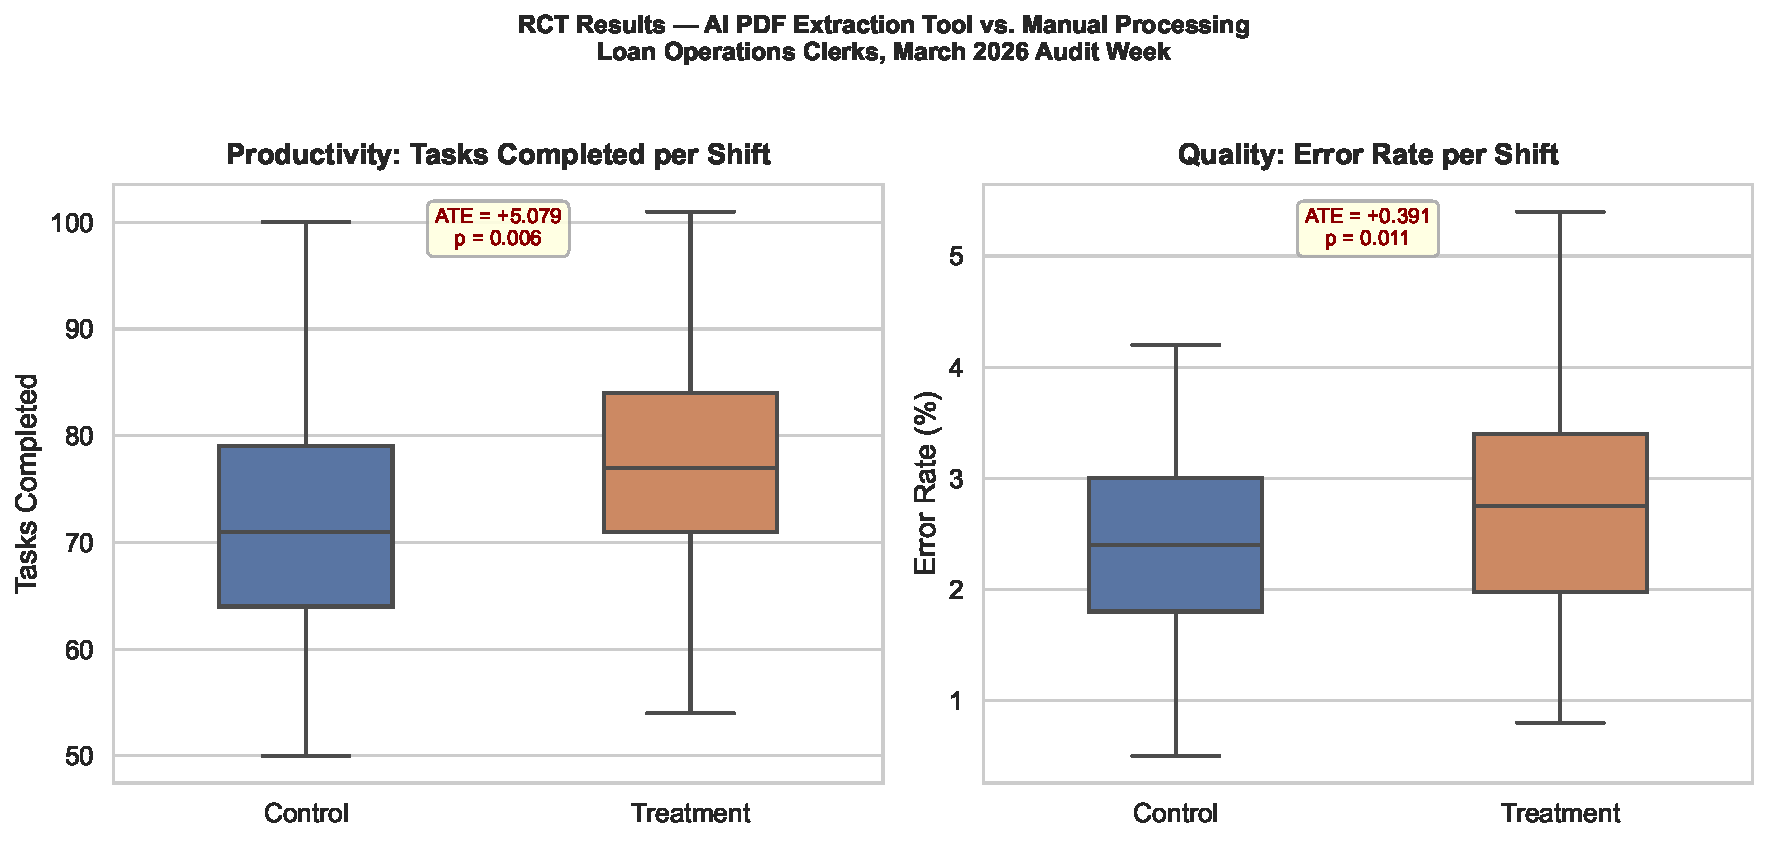
\includegraphics[width=\textwidth]{boxplots.pdf}
    \caption{Distribution of Tasks Completed (left) and Error Rate (right)
             by group. Treated clerks process more applications per shift
             but also produce more errors, consistent with a speed-accuracy
             trade-off induced by AI-assisted pre-filling.}
    \label{fig:boxplots}
\end{figure}

% ─────────────────────────────────────────────────────────────
\section{Interpretation}
\label{sec:interpret}

\textbf{What was the estimated marginal productivity gain?}
The AI PDF extraction tool produced an Average Treatment Effect of
\textbf{+5.08 additional tasks per shift} (95\% CI: $[1.52,\;8.64]$; $p = 0.006$).
Against a control group mean of 72.18 tasks, this represents a \textbf{7.0\% productivity
uplift} that is both statistically significant and operationally meaningful. At scale,
a one-week deployment across a 100-clerk operation translates to approximately 2,500
additional loan applications processed with no increase in headcount.

\textbf{Did the AI tool improve quality, or was there a quantity-quality trade-off?}
The data reveal a \textbf{quantity-quality trade-off}. The treatment group's error rate
was 0.39 percentage points higher than the control group (2.73\% vs.\ 2.34\%;
$p = 0.011$) --- a statistically significant quality penalty, not noise. The AI tool
appears to accelerate throughput in a way that invites automation complacency: when
the tool pre-fills fields, clerks may reduce per-item verification effort, accepting
AI outputs without sufficient scrutiny. This pattern is well-documented in the
human-automation teaming literature and is a non-trivial concern in regulated
financial environments where processing errors carry compliance and remediation costs.

\textbf{Implications for firms.}
These findings complicate the business case for broad AI deployment in loan operations.
The productivity gain is real and causally identified, but it arrives with a quality
cost firms cannot ignore. A thoughtful deployment strategy should pair the AI tool
with structured verification checkpoints, differentiated rollout by loan complexity
(e.g., Personal loans first, Mortgage last given higher error sensitivity), and
incentive structures that reward accuracy alongside throughput. Critically, the
randomized design used here provides a replicable blueprint: firms should embed
ongoing field experimentation rather than treating rollout as a one-time decision,
continuously re-estimating the productivity-quality trade-off as adoption matures
and workers calibrate their reliance on AI suggestions.

% ─────────────────────────────────────────────────────────────
\vspace{2em}\hrule\vspace{0.5em}
\footnotesize
\textit{All analysis code is in \texttt{analysis.py}. Figures and tables were generated
by running \texttt{python analysis.py} and are included above. The \texttt{AI-Lab}
GitHub repository (\texttt{yuweih13-debug}) contains four commits: Scrape, Clean,
Analyze, and Interpret.}

\end{document}
